\chapter{Experiments and Results} % Main chapter title


\lhead{Chapter 9. \emph{Robot Teacher Results}} % Change X to a consecutive number; this is for the header on each page - perhaps a

\label{chapter:teacher_results} % Change X to a consecutive number; for referencing this chapter elsewhere, use \ref{ChapterX}

In this chapter, we present a user study performed the capacity of our system to adapt plan explanation and management to the human's knowledge in the tasks to perform. Section~\ref{sec:teacher_results-scenario} presents our scenario. Section~\ref{sec:teacher_results-user_study} explains how we created and conducted our user study. Finally, section~\ref{sec:teacher_results-results} presents and discusses our results. This study was presented before in~\cite{milliez2016using}.



 \section{Scenario}
\label{sec:teacher_results-scenario}
To test our system, we have chosen a scenario where a human is trying to prepare two desserts, an apple pie and a banana pie, without knowing their recipes. The robot's goal is to teach the human how to prepare the two dishes, by explaining him the tasks that he has to execute, and by guiding him during this process, as shown in figure \ref{fig:teacher_results-scenario}. 

\begin{figure}[ht!]

 \centering
 \begin{tabular}{cc}
  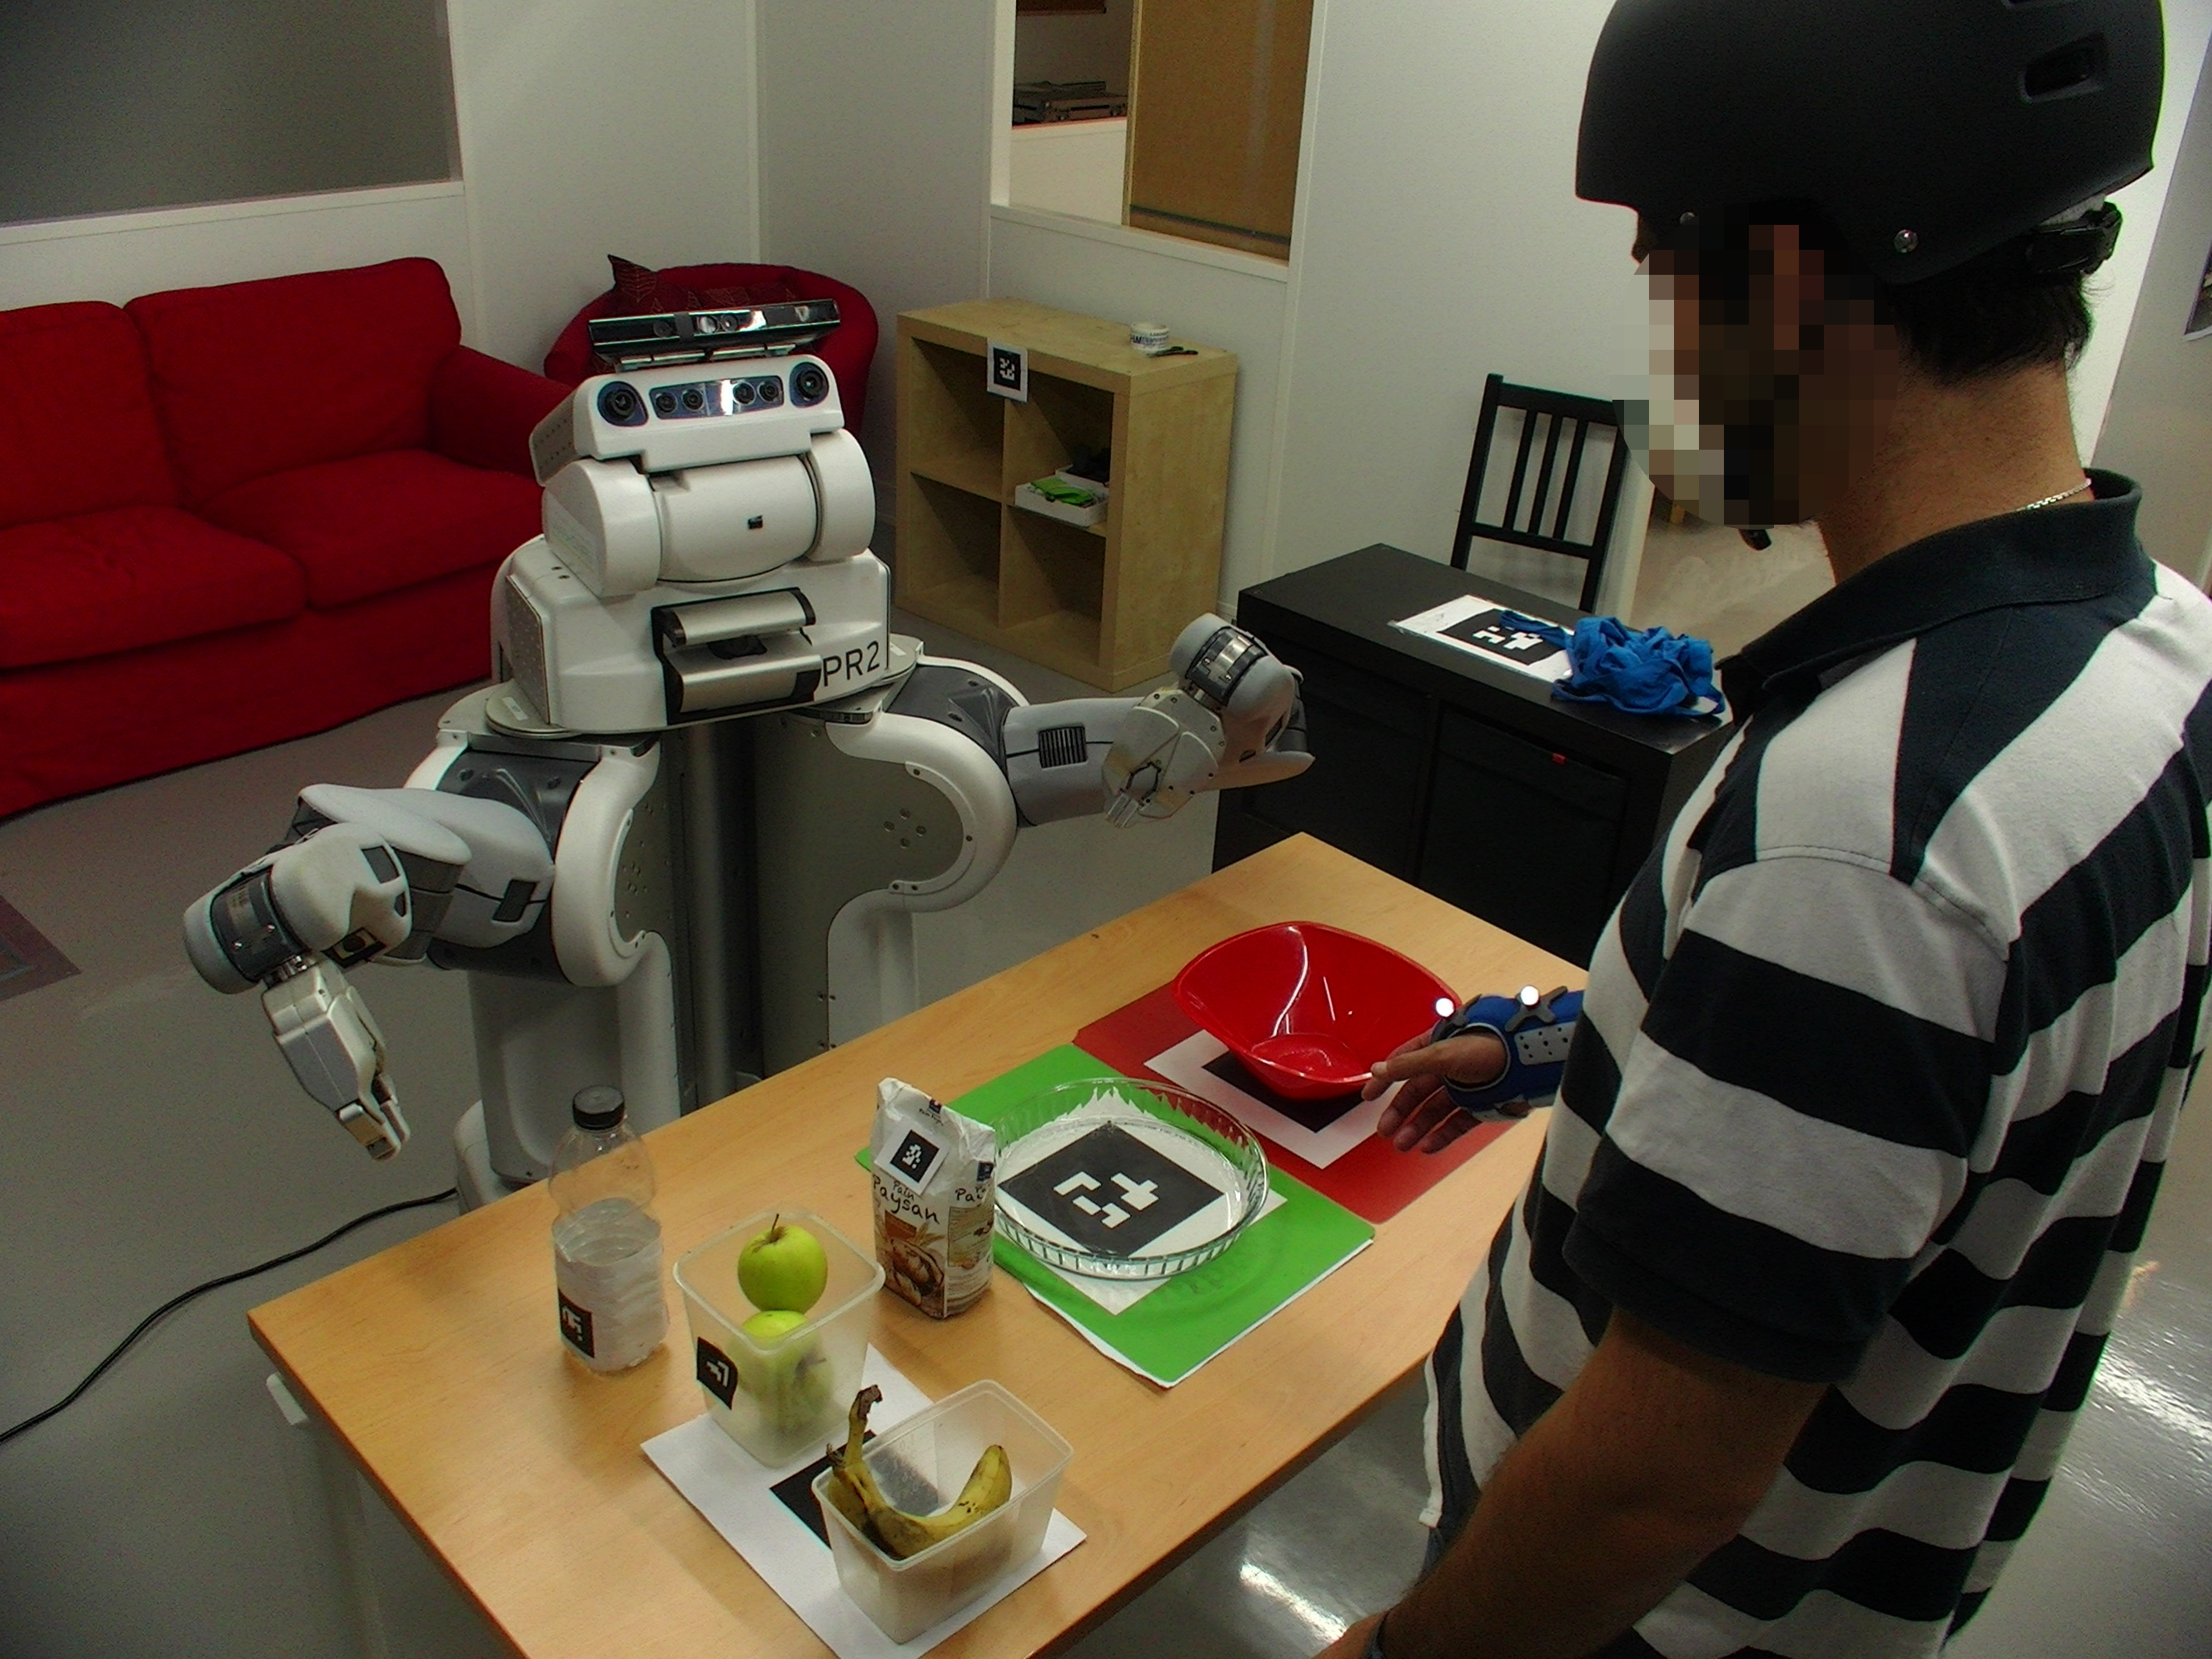
\includegraphics[width=0.29\textwidth]{img/teacher/scenario.JPG}
 \end{tabular}
 \caption{Illustration of the cooking pies scenario}
 \label{fig:teacher_results-scenario}
 \end{figure}

We created a domain to represent this scenario, and used it with the previously explained \textit{efficiency policy} and HATP as task planner. The process of cooking an apple pie involves five main tasks. We will now present an example of a simulated run in this scenario, to show how our algorithms would perform in this domain. In this example, we set the world state and chose which activities the human performs at each time.

 We imagine that, in our set-up, the robot is not able to execute the \textit{PrepareDough} and \textit{PrepareFruits} tasks, since it can not reach the needed ingredients. HATP produces a plan, allocating the tasks as follows:

\afterpage{\clearpage}
\begin{sidewaysfigure}[ht!]
 \centering
 \begin{tabular}{cc}
  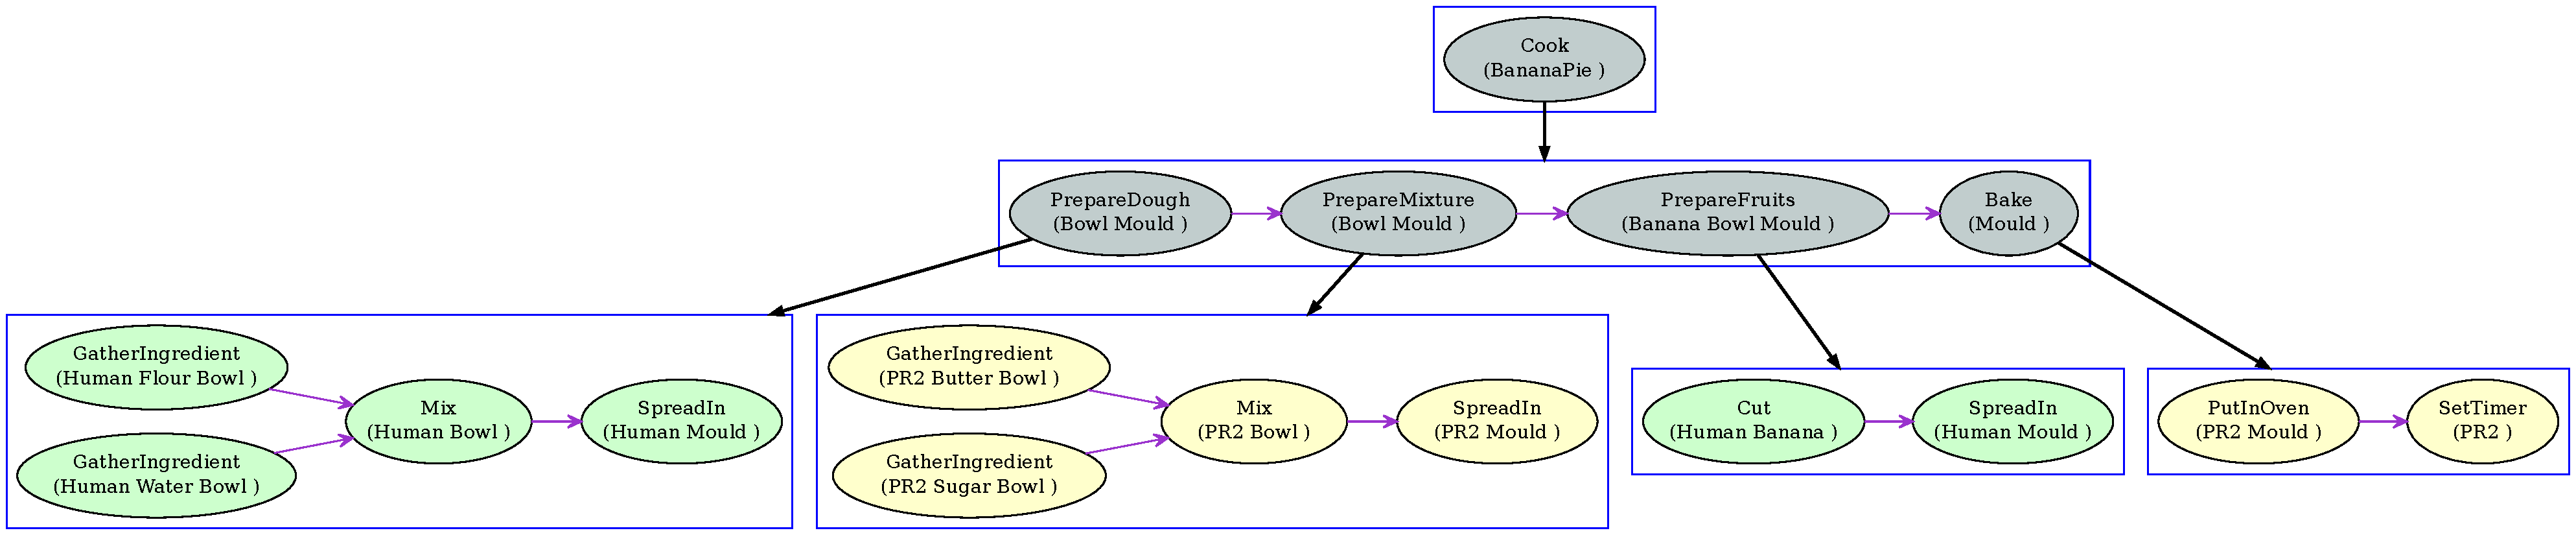
\includegraphics[scale=0.4]{img/teacher/bananaPie.pdf}
 \end{tabular}
 \caption{Shared plan generated to collaboratively make a banana pie.}
 \label{fig:teacher_results-bananaPlan}
 \end{sidewaysfigure}
 

\begin{enumerate}
\item The human will prepare the dough, kneading it and putting it in the mould.
\item The robot will prepare a mixture with butter and sugar, putting the ingredients in the mould.
\item The human will then prepare the required fruits, cutting them and adding them to the mixture..
\item Then, the human will prepare the dough for the top of the pie.
\item Finally, the robot will bake the pie, by putting it into the oven and setting a timer.
\end{enumerate} 

After completing task 1, the human's knowledge on how to prepare the dough will be improved. Consequently, during the execution of task 4, the robot will ask the user if he needs help to prepare the second dough. We imagine he answers ``no". The robot does not explain the task  and the system will upgrade the human's knowledge level for the \textit{PrepareDough} task to  \textit{intermediate}, after he completes its execution. The human's knowledge of task 3, \textit{PrepareFruit}, will be represented as \textit{human1 PrepareFruits [fruit] VALUE}. We consider the parameter of this task as \textit{class-link} , since the process will be the same for any fruit (cutting and putting in the mould). This way we use, as parameter, the class \textit{fruit} instead of the actual instances used in the task, \textit{apple} or \textit{banana}.

After cooking the first pie, the robot generates a plan to cook the banana pie. This time, we set the environment in order to allow  each agent to perform all the tasks. Preparing a banana pie is a similar process to the apple pie. The parameters will, of course, be different, involving bananas and not apple. Also, the banana pie does not have a second dough on its top, and it has a different baking time from the apple pie. The plan generated is presented in figure~\ref{fig:teacher_results-bananaPlan}. We can observe that the planner took into account the experience acquired by the human when preparing the apple pie, by assigning him the tasks (\textit{PrepareDough} and \textit{PrepareFruits}). During execution, since the user has an \textit{intermediate} knowledge level on \textit{PrepareDough}, the robot will not explain it. When the human is about to execute \textit{PrepareFruits}, the robot will propose to explain him the task, since he only performed it once, and has a \textit{beginner} knowledge level on it.


\section{User Study}
\label{sec:teacher_results-user_study}
We have conducted a comparative user study in order to have a first evaluation of our system's adaptability by users. Two groups of users were asked to participate in the two-pies scenario. The first group interacted with a simulated robot equipped with a basic system (BS). BS has the same behavior as our system, excluding the agent knowledge awareness mechanisms. The second group interacted with another system, which we will call knowledge system (KS), that exhibits similar characteristics to the presented system.

The hypothesis of our study is that, on average, users will express a preference on KS over BS. More formally, we set our null $H_0$ and alternative $H_A$ hypotheses as follows:
\begin{itemize}
\item $H_0$: $\mu_{KS}-\mu_{BS}=0$ 
\item $H_A$: $\mu_{KS}-\mu_{BS} \neq 0$  
\end{itemize}
where $\mu_{KS}$ and $\mu_{BS}$ are the average preference of users for the KS and BS systems.

In both systems, we generated a plan for the users which uses the same task  allocation presented in section~\ref{sec:teacher_results-scenario} to make an apple pie. For cooking a banana pie, KS will use the plan presented in figure~\ref{fig:teacher_results-bananaPlan}, where the human performs tasks he has already executed while preparing the apple pie. In BS, instead, we generated a plan that does not take into account human knowledge, and allocated tasks differently, by making the human prepare the mixture instead of the dough.

Two groups of 19 participants, from 18 to 60, interacted with each system in an online user study\footnote{User study for KS http://goo.gl/forms/qvbtu4vcFW, and BS http://goo.gl/forms/ZSvGcCi5le}, where we presented pictures of the task state and recordings of the robot's speech, in French, for each step of the interaction (as shown in figure~\ref{fig:teacher_results-user_study}).
At some steps, the user could choose the action to perform, allowing him to execute a wrong action, leading to a replan from the robot. For simplicity, the replan just corrected the wrong action, before resuming the previous plan. 
At the end of the simulated interaction, we have asked the same questions to both groups, concerning the adaptability of the system and the robot partner itself. 
The users gave marks along a Likert scale from one (disagree) to five (agree) to express their agreement with several statements (as shown in figure \ref{fig:teacher_results-user_study}).

\begin{figure}[ht!]
 \centering
 \begin{tabular}{cc}
  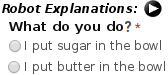
\includegraphics[width=0.24\textwidth]{img/teacher/ustudy9.png} &
  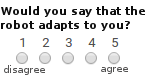
\includegraphics[width=0.19\textwidth]{img/teacher/ustudy11.png}
 \end{tabular} 
 \caption[User studies on plan adaptation]{\textit{Left}: The user listens to a recorded robot explanation and chooses the action to take. \textit{Right}: At the end, the user evaluates the interaction using a Likert scale.}
 \label{fig:teacher_results-user_study}
 \end{figure}

\section{Results and Discussion}
\label{sec:teacher_results-results}

We collected the answers from each form, and computed the mean, along with the standard deviation and p-value to evaluate the system. The p-value was computed using a t-distribution with 18 degrees of freedom and evaluated using a significance value $\alpha=0.05$.
%We compare below the results for each system. 
Figure~\ref{fig:teacher_results-results} summarizes the results. Comparing users' answers, we can see that users appreciated the capacity of the system to explain the plan while adapting to their knowledge, with a mean of 3.74 for KS against 2.05 for BS. The users interacting with KS globally noticed that the task distribution took their knowledge into account, by giving a mean rating of 3.42 for KS and 2.58 for BS. The last question concerned the freedom to choose how to perform the task. In this case, the calculated mean was 2.58 for KS and 1.89 for BS. In all these cases, the p-value was lower than the $\alpha$. 

With KS, the users attributed a mean of 3.11 for the global adaptability of the system against 1.89 for the basic one.
We also asked how the robot partner was perceived. While in KS the robot is not perceived as more verbose (2.53 for KS against 2.47 for BS), people found the interaction slightly more natural (2.74 against 2.42) and the robot appeared smarter (2.79 against 2.26). Even if these last two results look favorable, since their p-value is higher than $\alpha$  we do not have enough evidence to prove a difference between the two systems. We believe that other aspects might have been taken into account by the users, such as the speech itself, which conditioned their perception on the naturalness of the interaction. Improving the robot's verbalization process with a synonym dictionary could be a first step to get more significant results.



 \begin{figure}[ht!]
 \centering
 \begin{tabular}{cc}
  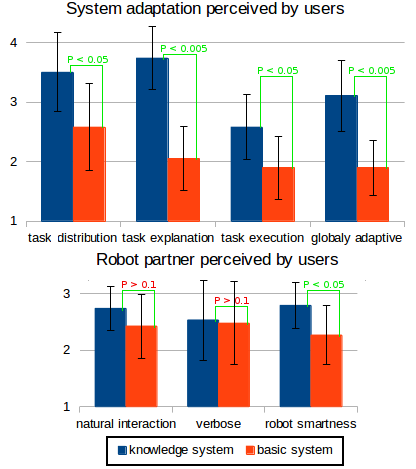
\includegraphics[width=0.45\textwidth]{img/teacher/respvalue3.png}
 \end{tabular}
 \caption[Average users' rating of the interaction on several criteria]{Average users' rating of the interaction on several criteria. Blue for KS and red for BS.}
 \label{fig:teacher_results-results}
 \end{figure}

This study sheds light on how users were able to perceive the robot adaptation to their knowledge concerning task distribution, task explanation and monitoring. In addition, the robot partner was perceived as smarter and the interaction seemed a bit more natural to the users. However, these first results need to be confirmed with study on a larger population. Also, as the scenario was simulated, results on a real robot might differ.
In both studies, we asked the participants how the system could be improved. Several users suggested they would like to be able to choose which action to perform, showing the importance of negotiation. A user suggested he would like to be informed about the progress of the task from time to time. Other comments concerned suggestions about the robot's speech capacities, like its voice, intonation, and the chosen words. These aspects were not the aim of our  experiment but are indeed an important part of the interaction process. 
